\documentclass[presentation]{beamer}
\usepackage{oop-slides}
\setbeamertemplate{bibliography item}[text]
\newcommand{\lessonnr}[0]{06}
\title[OOP09 -- Deployment and Concurrency]{09\\Deployment di applicazioni, Programmazione multipiattaforma, Profiling e Concorrenza}

\begin{document}

\frame[label=coverpage]{\titlepage}

%====================
%Outline
%====================
\begin{frame}<beamer>
 	\frametitle{Outline}
 	\tableofcontents[]
\end{frame}

\begin{frame}{``Write once, run anywhere...''}
Lo ``slogan'' coniato originariamente da \textit{Sun Microsystems} per illustrare i benefici del linguaggio Java vale a patto che:

\begin{enumerate}\itemsep10pt
\item \textbf{``write'' sia fatta in modo corretto e robusto},
\begin{itemize}
\item ovvero, sia adottato un approccio di programmazione adeguato.
\end{itemize}
\item \textbf{sia possibile distribuire ciascuna applicazione per qualunque piattaforma}.
\begin{itemize}
\item ovvero, sia predisposto un deployment efficace. 
\end{itemize}
\end{enumerate}
\end{frame}

\section{Programmazione multipiattaforma}

\subsection{Accesso al file system}
\begin{frame}{Path e Separatori}
Inserire dei path assoluti nel proprio sorgente è \textbf{sempre} fonte di problemi quando si scrive software multipiattaforma:
\begin{itemize}
\item \url{C:\\Users\\UserName\\file} --- Non funzionerà su piattaforma *nix, e non funzionerà se l'utente Windows non è ``UserName''.

\item \url{C:\\MyProgram\\file} --- Non funzionerà su piattaforma *nix, e non funzionerà se l'installazione di Windows è sana e il software non è avviato come admin.

\item \url{/home/username/file} --- Non funzionerà su piattaforma Windows, e non funzionerà se l'utente non è \texttt{username}.
\end{itemize}

\begin{block}{Problemi}
\begin{itemize}
\item I separatori per i path cambiano a seconda dell'OS!
\item La struttura del file system cambia con l'OS!
\item I diritti di lettura e scrittura cambiano con la configurazione.
\end{itemize}
\end{block}
\end{frame}

\begin{frame}{Proprietà di sistema}
Java fornisce nella classe \texttt{System} un metodo\\
\begin{center}
{\Large \texttt{String getProperty(String par)}}
\end{center}
che consente di accedere a proprietà di sistema in modo corretto!
\vspace{10pt}
\begin{block}{Alcuni parametri ammissibili}
\begin{itemize}
\item \texttt{file.separator} --- Restituisce \url{\\} per Windows e \url{/} per Unix
\item \texttt{java.home} --- La directory di installazione di Java
\item \texttt{user.dir} --- La directory da cui il comando \texttt{java} è stato invocato
\item \texttt{user.home} --- Restituisce la home directory dell'utente che ha lanciato \texttt{java}
\item \texttt{user.name} --- Restituisce il nome utente
\end{itemize}
\end{block}
\end{frame}

\begin{frame}{Funzionalità OS-specifiche}
\begin{itemize}\itemsep10pt
\item Talvolta è possibile che in una applicazione si debbano utilizzare librerie non disponibili o non licenziate per alcune piattaforme.
\item A supporto di ciò, Java fornisce delle proprietà che consentono di identificare OS, versione e JVM corrente.
\end{itemize}

\begin{block}{Altri parametri ammissibili}
\begin{itemize}
\item \texttt{java.version} --- La versione di \texttt{java} in uso. Si potrebbe decidere di non usare una funzionalità che si sa non esistere o essere buggata.

\item \texttt{os.arch} --- L'architettura della CPU come rilevata dall'OS (es. x86, i386, amd64, x86\_64, IA64N, arm,\dots)

\item \texttt{os.name} --- Il nome del sistema operativo (es. Linux, MacOS X, MacOS, Windows 8.1, Windows 10, Solaris, FreeBSD, \dots)

\item \texttt{os.version} --- Restituisce per Windows il numero di versione effettivo (es. Windows 10 restituisce 10.0), per MacOS il numero di versione (es. 10.3.4), per Linux la versione del kernel (es. 3.17)
\end{itemize}
\end{block}

\end{frame}


\subsection{Font ed encoding}

\begin{frame}{Font ed encoding}
Le più note piattaforme utilizzano di default encoding diversi:

\begin{itemize}
\item \textbf{UTF-8} --- default su Linux, può essere considerato lo standard de-facto.
\item \textbf{MacRoman} --- default su MacOS, raramente causa artefatti se riconvertito ad altri formati.
\item \textbf{ISO-8859-1} --- default su Windows, può causare artefatti su quasi tutti i caratteri non ASCII se convertito a UTF-8.
\end{itemize}

\begin{block}{Encoding per il codice sorgente}
Solitamente, il codice sorgente si sviluppa utilizzando la codifica UTF-8
\begin{itemize}
\item Essenziale se si utilizzano caratteri non inclusi nella tabella ASCII (caratteri accentati, ad esempio).
\end{itemize}
\end{block}
\end{frame}

\begin{frame}{Uso di UTF-8 in Eclipse}
$\rightarrow$ Windows $\rightarrow$ Preferences $\rightarrow$ General $\rightarrow$ Workspace $\rightarrow$ Text file encoding $\rightarrow$ Other $\rightarrow$ UTF-8 $\rightarrow$ OK
\begin{center}
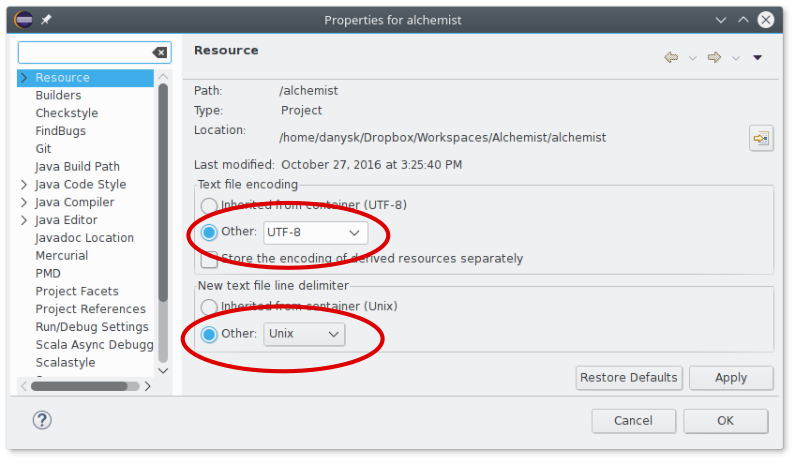
\includegraphics[width=0.7\textwidth]{img/eclipse-encoding}
\end{center}
\end{frame}

\subsection{GUI scalabili}

\begin{frame}{GUI scalabili -- Motivazioni}
\begin{block}{Flessibilità}
Diversamente dagli anni 90, i dispositivi oggi hanno una densità di pixel per area \textbf{estremamente} variabile. Si va da 120 PPI a 640 PPI, su schermi di dimensione estremamente variabile (da 3 a 200 pollici).
\end{block}

\begin{block}{Multipiattaforma}
Piattaforme diverse, anche a parità di schermo, possono adottare diverse convenzioni:
\begin{itemize}
\item Diversa grandezza di bordi
\item Diversa spaziatura, dimensione e tipo di font
\item Diverso sistema di decorazioni
\end{itemize}

Questi elementi sono stabiliti dal \emph{compositor} e non dallo sviluppatore dell'applicazione. Come indicazione generale vale che \textbf{un'applicazione ben sviluppata eredita il ``look and feel'' dal sistema su cui sta girando}.
\end{block}
\end{frame}

\begin{frame}{Esempio: Finestra non ridimensionabile e bassa risoluzione}
\centering
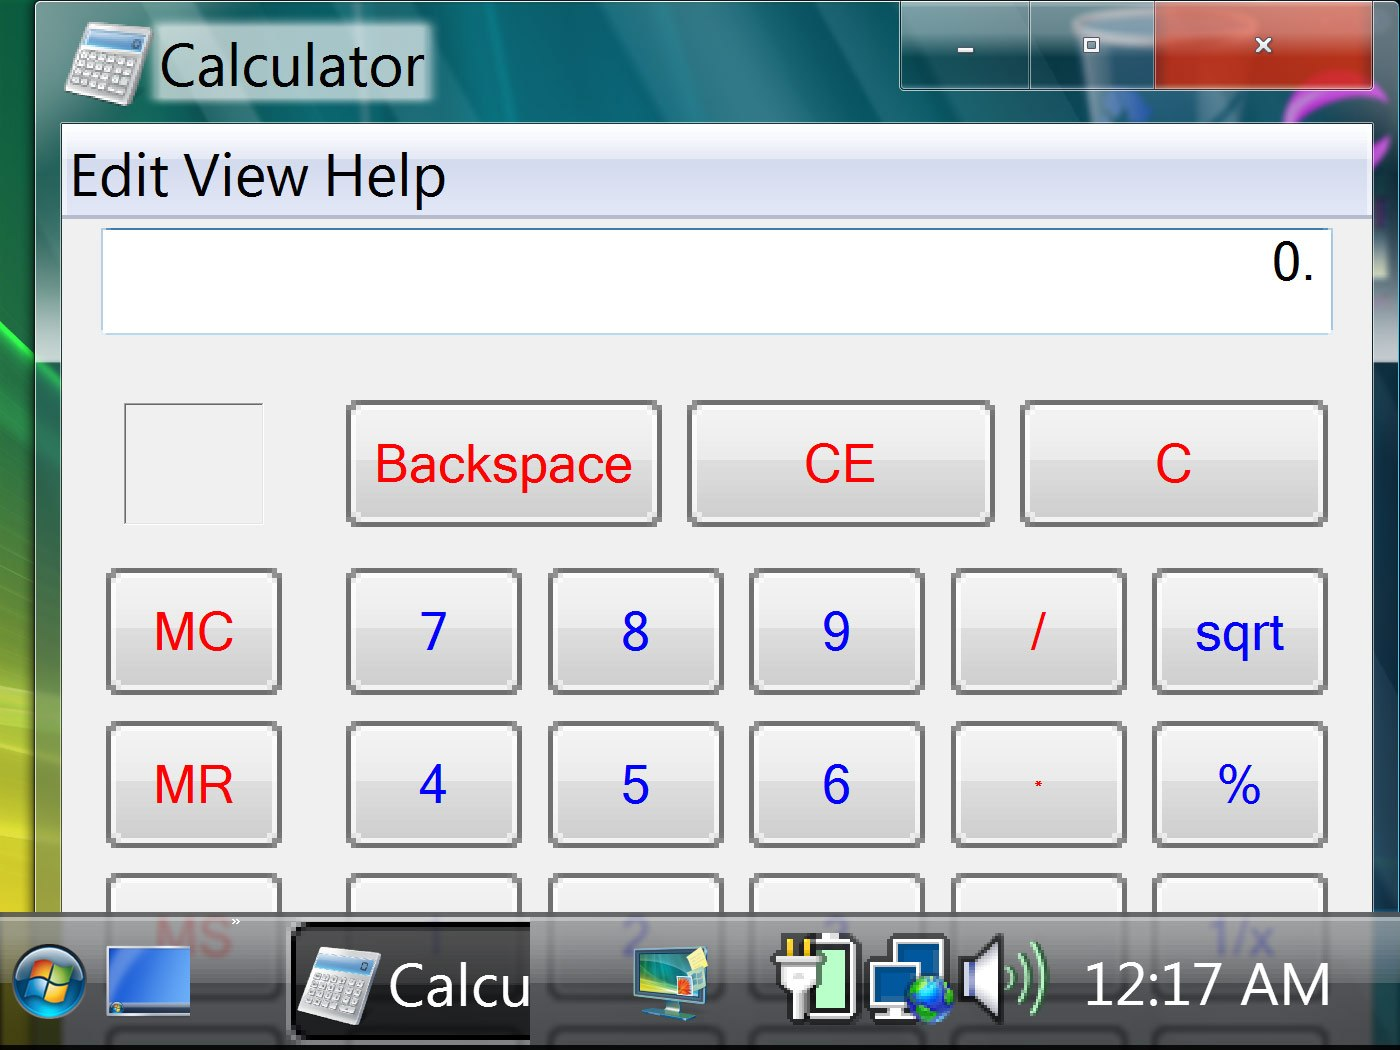
\includegraphics[width=0.8\textwidth]{img/lowres}
\end{frame}

\begin{frame}{Esempio: Finestra non ridimensionabile e alta risoluzione}
\centering
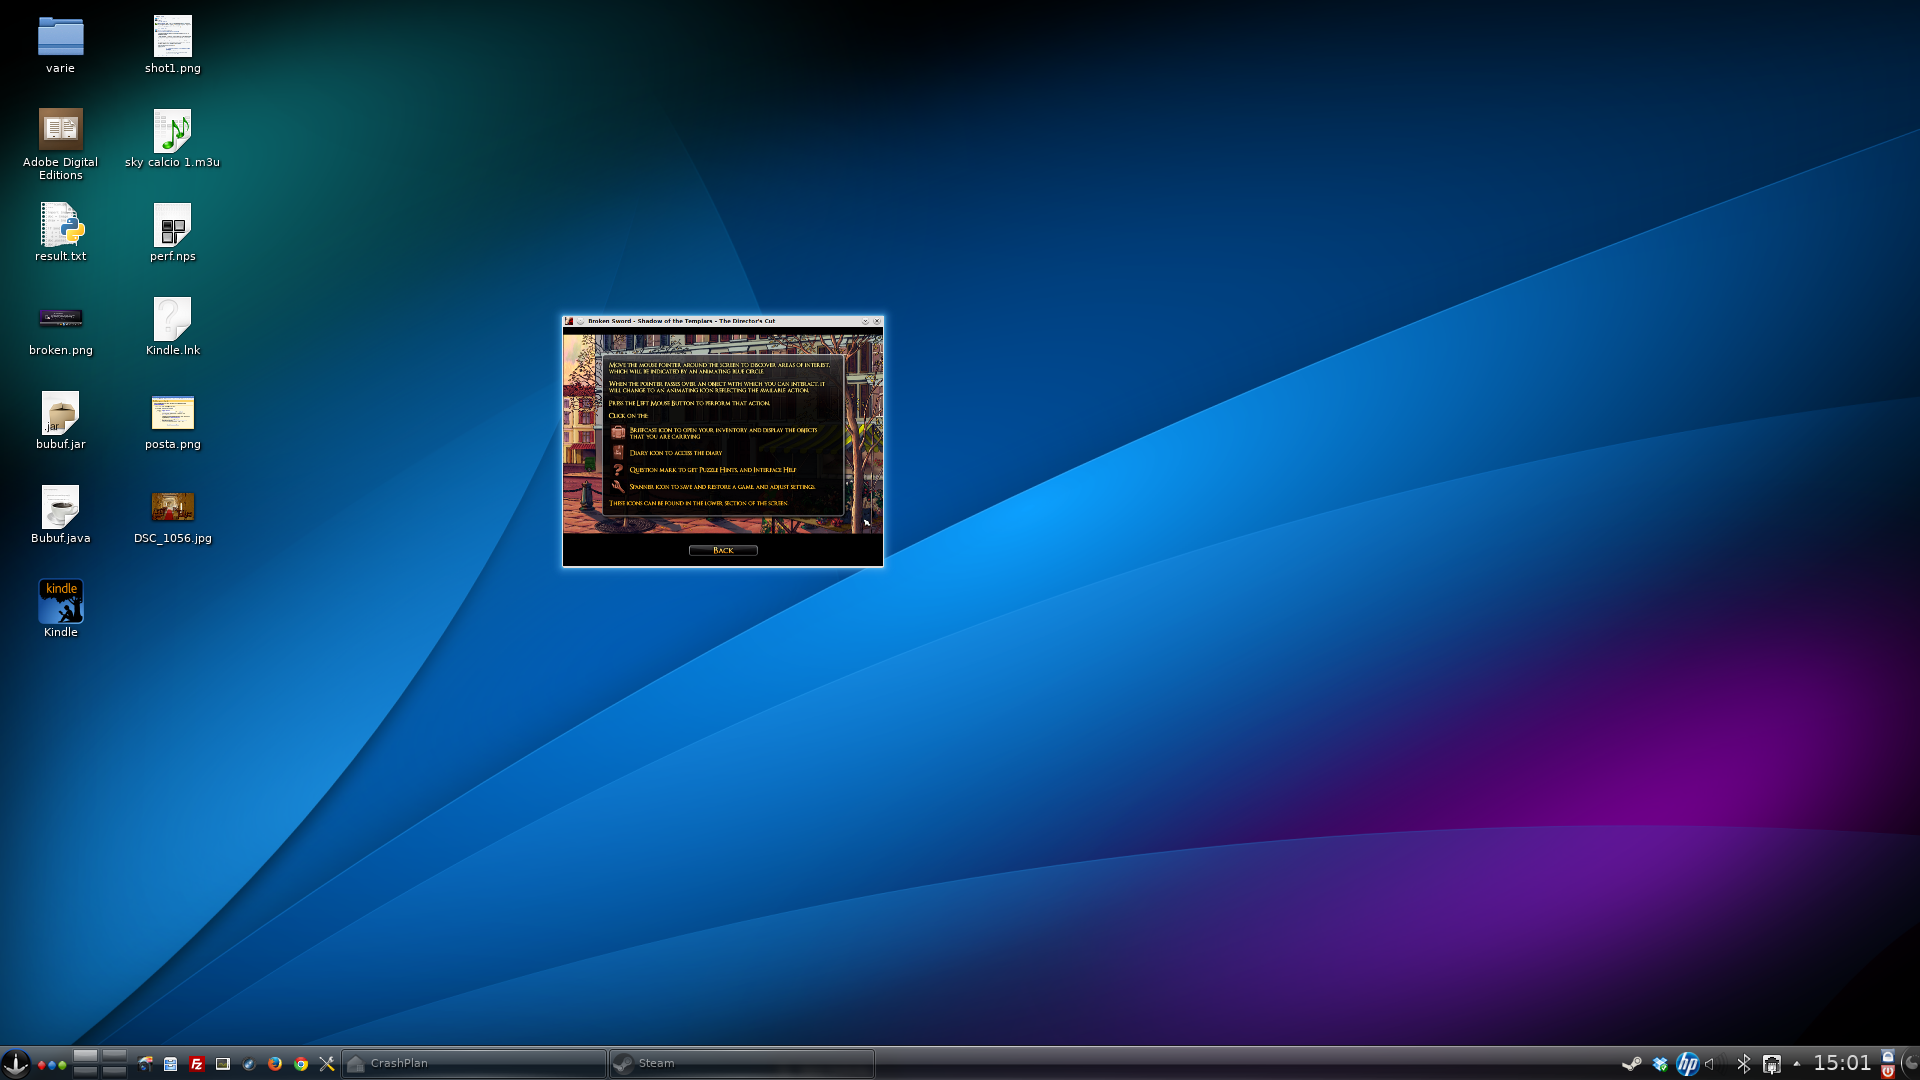
\includegraphics[width=0.8\textwidth]{img/brokensword}
\end{frame}

\begin{frame}{Best-practices per la costruzione di GUI}
\begin{itemize}\itemsep10pt
\item La dimensione di default della finestra va calcolata in base alla dimensione dello schermo.
\item \`{E} opportuno \underline{non} specificare dimensioni assolute in pixel per i componenti della GUI, ma dimensionarli in termini relativi rispetto al container.
\item Anche per i layout è opportuno non utilizzare dimensioni fisse in pixel.
\item Preferire i font di sistema (la JVM in automatico associa il font di default dell'OS).
\item Preferire la dimensione dei font di default, se se ne sceglie una diversa, renderla relativa alla dimensione corrente della view.
\end{itemize}
\end{frame}

\subsection{Supporto all'internazionalizzazione}

\begin{frame}{Supporto multilingua per le GUI}
\begin{itemize}
\item Sarebbe opportuno definire la GUI una sola volta e cambiare dinamicamente le parti scritte (il testo) a seconda dell'impostazione della lingua di sistema (o della nostra applicazione).
\begin{itemize}
\item In realtà, non solo per la lingua ma anche per il formato dei numeri, la valuta, le convenzioni sulla data,\dots
\end{itemize}
\end{itemize}
\begin{block}{Java Resource Bundles}
Java fornisce una architettura per l'internazionalizzazione, che fa uso di ``\textbf{ResourceBundle}'' e di una serie di file di supporto (properties files).

Per approfondimenti (per implementare il supporto multilingua):
\begin{itemize}
\item \url{https://docs.oracle.com/javase/tutorial/i18n/resbundle/index.html}
\item \url{http://tutorials.jenkov.com/java-internationalization/resourcebundle.html}
\end{itemize}
\end{block}
\end{frame}

\section{Deployment di applicazioni}

\begin{frame}{Deployment: indicazione generale}
\begin{itemize}\itemsep20pt
\item \textbf{Per le applicazioni scritte in linguaggio Java, è buona norma distribuire un archivio JAR eseguibile autocontenuto.}
\begin{itemize}
\item In Eclipse: (Project dir) $\rightarrow$ Export... $\rightarrow$ Java $\rightarrow$ Runnable JAR File
\end{itemize}
\item Esistono anche setup diversi, ad esempio con installer dedicati per ciascuna piattaforma, che aggiungono notevole complessità e tempo senza nessun vantaggio realmente importante.
\end{itemize}

\end{frame}

\subsection{Corretta configurazione di un progetto Eclipse}

\begin{frame}{Corretta struttura di un progetto}
\centering
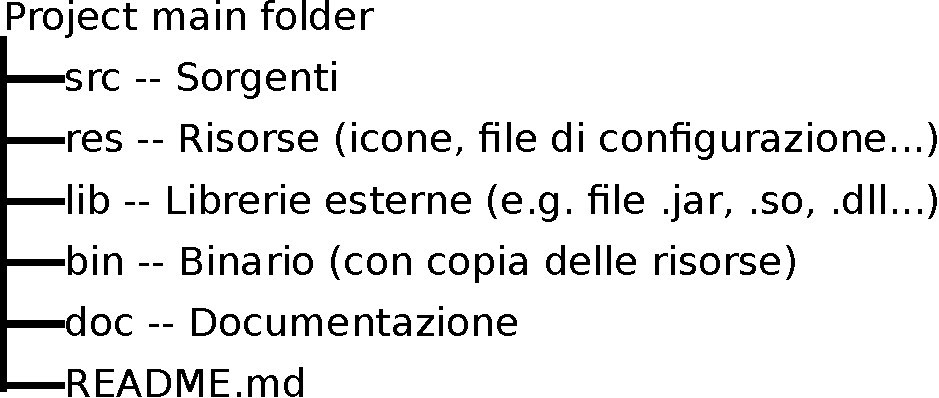
\includegraphics[width=0.99\textwidth]{img/struct}
\end{frame}

\begin{frame}{Corretta struttura di un progetto -- Dettagli (1/3)}

\begin{block}{\texttt{src}}
\begin{itemize}
\item Contiene \textbf{esclusivamente} il codice sorgente dell'applicazione organizzato in package. Non deve contenere altro!

\item Eventualmente possono esistere più cartelle sorgente.
\begin{itemize}
\item Ad esempio perché parte del codice viene generato da un sistema automatico, oppure perché il progetto è sviluppato usando più di un linguaggio.
\item Nel caso di generatori, è buona norma dividere il codice generato da quello generante, ad esempio creando una cartella \texttt{src-gen}.
\item Nel caso si utilizzino più linguaggi, è bene distinguerli usando source folder separate, es. \texttt{src-java} e \texttt{src-prolog}.
\end{itemize} 

\item In Eclipse è possibile marcare una cartella come ``cartella sorgente'': Proprietà del progetto $\rightarrow$ Java Build Path $\rightarrow$ Source $\rightarrow$ Add Folder $\rightarrow$ Selezione della cartella $\rightarrow$ OK $\rightarrow$ OK
\begin{itemize}
\item Tutti i sorgenti di tutte le cartelle sorgente verranno compilati ed inseriti nella cartella di output da Eclipse
\end{itemize}		
\end{itemize}
\end{block}
\end{frame}

\begin{frame}{Corretta struttura di un progetto -- Dettagli (2/3)}
\begin{block}{\texttt{res}}
\begin{itemize}
\item Contiene le risorse del progetto opportunamente organizzate
\begin{itemize}
\item Per risorse si intendono icone, file di testo, video, immagini, modelli 3D e qualunque cosa sia necessaria al corretto funzionamento del programma ma non sia una libreria o un file sorgente.
\end{itemize}

\item In Eclipse, per far sì che le risorse vengano inserite nel classpath (da cui sarà più facile caricarle), è necessario rendere \texttt{res} una cartella sorgente con la procedura descritta nella slide precedente.
\end{itemize}
\end{block}

\begin{block}{\texttt{lib}}
\begin{itemize}
\item	Contiene tutte le librerie che si sono usate, che siano in file jar o che siano librerie native in formato .so (o .dll)
\end{itemize}
\end{block}
\end{frame}

\begin{frame}{Corretta struttura di un progetto -- Dettagli (3/3)}
\begin{block}{\texttt{doc}}
\begin{itemize}
\item Contiene la documentazione del progetto.
\item Sesi decide di inserire sia documentazione di tipo non rigenerabile (e.g. una relazione in pdf) sia quella di tipo rigenerabile (e.g. la javadoc), è bene tenerle separate (facilita il tracking con DVCS).
\end{itemize}
\end{block}

\begin{block}{\texttt{bin}}
\begin{itemize}
\item Contiene la versione compilata del vostro software.
\item In Eclipse, la creazione di questa cartella è compito del SDK.
\end{itemize}
\end{block}

\begin{block}{\texttt{README.md}}
\begin{itemize}
\item File con la descrizione del progetto: autori, breve guida d'uso, link a risorse. \begin{itemize}
\item Bitbucket e GitHub sono in grado di fare il parse del file e di integrarlo nella pagina del progetto, in modo da dargli una descrizione.
\end{itemize} 
\end{itemize}
\end{block}

\end{frame}

\begin{frame}{Utilizzo di path relativi in Eclipse (1/2)}
\begin{itemize}\itemsep20pt
\item Quando si lavora ad un progetto, \textbf{è bene che tutti i path siano relativi alla radice del progetto stesso}.
\item In caso contrario:
\begin{itemize}
\item Gli altri membri del team dovranno continuamente cambiare le impostazioni per adattarle al loro file system.
\item Il progetto non sarà sviluppabile su piattaforme diverse.
\item Questo è vero in particolare per le librerie, supponendo che le risorse siano gestite correttamente.
\item \dots
\end{itemize}
\end{itemize}
\end{frame}

\begin{frame}{Utilizzo di path relativi in Eclipse (2/2)}

\begin{block}{Procedura \textbf{\underline{NON}} corretta}
Il modo \textbf{\underline{sbagliato}} di cui importare una libreria in Eclipse è: Proprietà del progetto $\rightarrow$ Java Build Path $\rightarrow$ Libraries $\rightarrow$ Add External JARs $\rightarrow$ Selezione dei JAR $\rightarrow$ OK $\rightarrow$ OK
\begin{itemize}
\item \`{E} possibile scegliere JAR da qualunque punto del file system.
\item Vengono generati percorsi assoluti.
\end{itemize}
\end{block}

\begin{block}{Procedura \textbf{\underline{corretta}}}
Il modo \textbf{\underline{corretto}} di cui importare una libreria in Eclipse è: Proprietà del progetto $\rightarrow$ Java Build Path $\rightarrow$ Libraries $\rightarrow$ Add JARs $\rightarrow$ Selezione dei JAR $\rightarrow$ OK $\rightarrow$ OK
\begin{itemize}
\item \`{E} possibile scegliere solo JAR file che esistono in una delle cartelle del progetto (e, se il progetto è ben configurato, sono inserite in \texttt{lib}).
\item Vengono generati percorsi relativi alla root del progetto.
\end{itemize}
\end{block}
\end{frame}

\subsection{Caricamento di risorse dal classpath}

\begin{frame}{Risorse caricate dal classpath}
\begin{itemize}
\item Abbiamo inserito le nostre risorse nel progetto in maniera tale che vengano copiate nella cartella bin.
\item Queste risorse ed i file compilati verranno anche inseriti nel JAR eseguibile.
\item Come possiamo accedere a queste risorse in modo trasparente?
\begin{itemize}
\item Ossia caricarle sia che si trovino sul file system, sia che si trovino nel JAR eseguibile, sia che vengano incluse in un JAR di risorse separato.
\end{itemize} 
\end{itemize}
\begin{block}{\texttt{Class.getResource()}}
\begin{itemize}
\item Java fornisce un'utilità per caricare risorse dal \textbf{classpath}
\item Come abbiamo visto usando l'opzione \texttt{-cp} di \texttt{java} e \texttt{javac}, il classpath può contenere indifferentemente dei path o dei JAR
\end{itemize}
\end{block}
\end{frame}

\begin{frame}[fragile]{Risorse caricate dal classpath -- Esempi}

\begin{block}{Caricamento di File}
\begin{lstlisting}
final InputStream in = LoadImage.class.getResourceAsStream("/settings/settings");
final BufferedReader br = new BufferedReader(new InputStreamReader(in));
final String line = br.readLine();
in.close();
\end{lstlisting}
\end{block}

\begin{block}{Caricamento di Immagini}
\begin{lstlisting}
final URL imgURL = LoadImage.class.getResource("/images/gandalf.jpg");
final ImageIcon icon = new ImageIcon(imgURL);
final JLabel lab1 = new JLabel(icon);
\end{lstlisting}
\end{block}
\end{frame}

\subsection{Installazione per-utente}

\begin{frame}{Installazione delle impostazioni}
\begin{block}{Motivazione}
Spesso un software ha necessità di caricare al primo avvio delle impostazioni di default, quindi lasciare l'utente libero di modificarle e, se avviato successivamente caricare quelle scelte dall'utente. In caso di sistema multiutente, le impostazioni saranno diverse per ciascuno.
\end{block}

\begin{block}{Strategia}
\begin{itemize}
\item Si sceglie una cartella nella home folder dell'utente dove salvare le impostazioni. 
\begin{itemize}
\item È norma consolidata creare una cartella \texttt{.nomeprogramma}.
\end{itemize}

\item Al primo avvio, si verifica se tale cartella esiste e se contiene i file di configurazione previsti.
\begin{itemize}
\item Se non è presente (o se non sono presenti alcuni/tutti) i file oppure se non sono leggibili), si procede a caricare nella cartella di destinazione i file di default usando \texttt{getResource()}.
\end{itemize}
\end{itemize}
\end{block}
\end{frame}

\section{Ricerca/Utilizzo di Librerie a Supporto}
\begin{frame}{Uso di Librerie a Supporto}
\begin{itemize}\itemsep15pt
\item Durante lo sviluppo di un software, spesso emerge la necessità di realizzare componenti a supporto della propria applicazione, utili per incapsulare un determinato comportamento/funzionalità ma non cruciali per la logica applicativa.

\item Nella maggior parte dei casi una tale libreria/componente è già stato sviluppato da qualcun altro!

\item Risulta opportuno avvalersi di librerie open source già disponibili e testate\dots
\begin{itemize}
\item \dots dopo aver letto attentamente la documentazione e averne compreso a fondo il comportamento!
\end{itemize}
\end{itemize}
\end{frame}

\begin{frame}{The Maven Central Repository}
\begin{itemize}\itemsep10pt
\item Costituisce la più ampia collezione di librerie e componenti Java open-source.
\begin{itemize}
\item È il repository di default per Apache Maven (il più noto tool per il project management).
\end{itemize}
\item Rappresenta uno dei modi più rapidi per accedere a librerie sviluppate da altri sviluppatori e distribuire le proprie.
\item Consente di ricercare e scaricare pressoché qualunque libreria a supporto utile nelle proprie applicazioni open-source.

\item \url{https://search.maven.org/}
\end{itemize}
\end{frame}

\begin{frame}{Top 20 Java Library}
\begin{center}
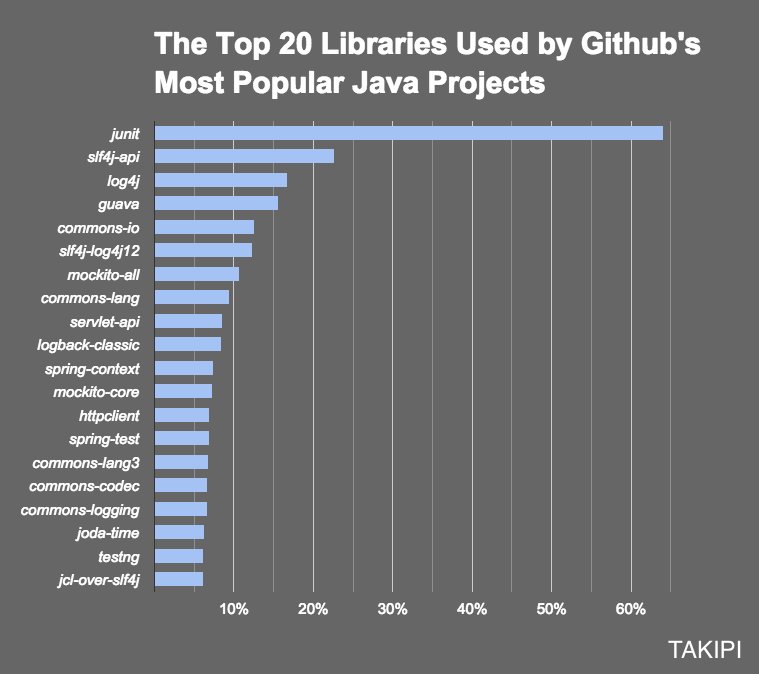
\includegraphics[width=0.6\textwidth]{img/top-20-java-libraries}
\end{center}
{\scriptsize \url{blog.takipi.com/we-analyzed-60678-libraries-on-github-here-are-the-top-100}}
\end{frame}

\begin{frame}{Altri Repository per librerie Java-based}
\begin{itemize}\itemsep15pt
\item \textbf{Google Guava} (\url{https://github.com/google/guava})
\begin{itemize}
\item Il progetto Guava di Google raccoglie diverse librerie core sviluppate da Google che possono essere utilizzate per lo sviluppo di applicazioni.
\item Ad esempio, sono disponibili librerie per Collections Management, Concurrency, I/O, String Processing,\dots
\end{itemize}
\item \textbf{Apache Commons} (\url{https://commons.apache.org})
\item \textbf{SLF4J} (\url{http://www.slf4j.org})
\begin{itemize}
\item Consente di utilizzare una serie di framework per il logging.
\end{itemize}
\end{itemize}
\end{frame}

\section{Esercitazione sulla concorrenza}

\subsection{JVisualVM}

\begin{frame}{Profiling di applicazioni Java}
\begin{itemize}\itemsep10pt
\item Quando si sviluppa un'applicazione complessa, soprattutto se basata su meccanismi di concorrenza, è opportuno analizzarne il comportamento e monitorarne le performance.
\begin{itemize}
\item Spesso il monitoraggio delle performance è essenziale per identificare eventuali problematiche o capire l'origine di problemi che possono essere insorti.
\end{itemize}
\item Tra gli strumenti che possono essere utilizzati per monitorare l'esecuzione di applicazioni che sono eseguite sulla JVM, due sono distribuiti unitamente al Java Development Kit (JDK).
\begin{itemize}
\item \textbf{JConsole}, lo storico (e scarno) tool per il profiling di applicazioni Java.
\item \textbf{JVisualVM}, il più recente ed evoluto tool utilizzabile per monitorare l'evoluzione e le performance di applicazioni in esecuzione sulla JVM.
\end{itemize}
\end{itemize}
\end{frame}

\begin{frame}{JVisualVM}
\begin{itemize}\itemsep10pt
\item Si tratta di un profiler per applicazioni Java che consente di misurarne ed analizzarne le performance.
\item Interagisce con la JVM per fornire informazioni circa le performance e il consumo di risorse di applicazioni in esecuzione.
\item Distribuito internamente al JDK dalla versione 5.0
\item Consente di monitorare:
\begin{itemize}
\item la percentuale di CPU utilizzata da singoli metodi, thread, \dots
\item per quanto tempo un thread si trova nello stato di running oppure in stato di blocco o di idle.
\item \dots
\end{itemize}
\item Richiamabile attraverso il comando \texttt{jvisualvm}.
\end{itemize}
\end{frame}

\begin{frame}{JVisualVM - Overview}
\centering
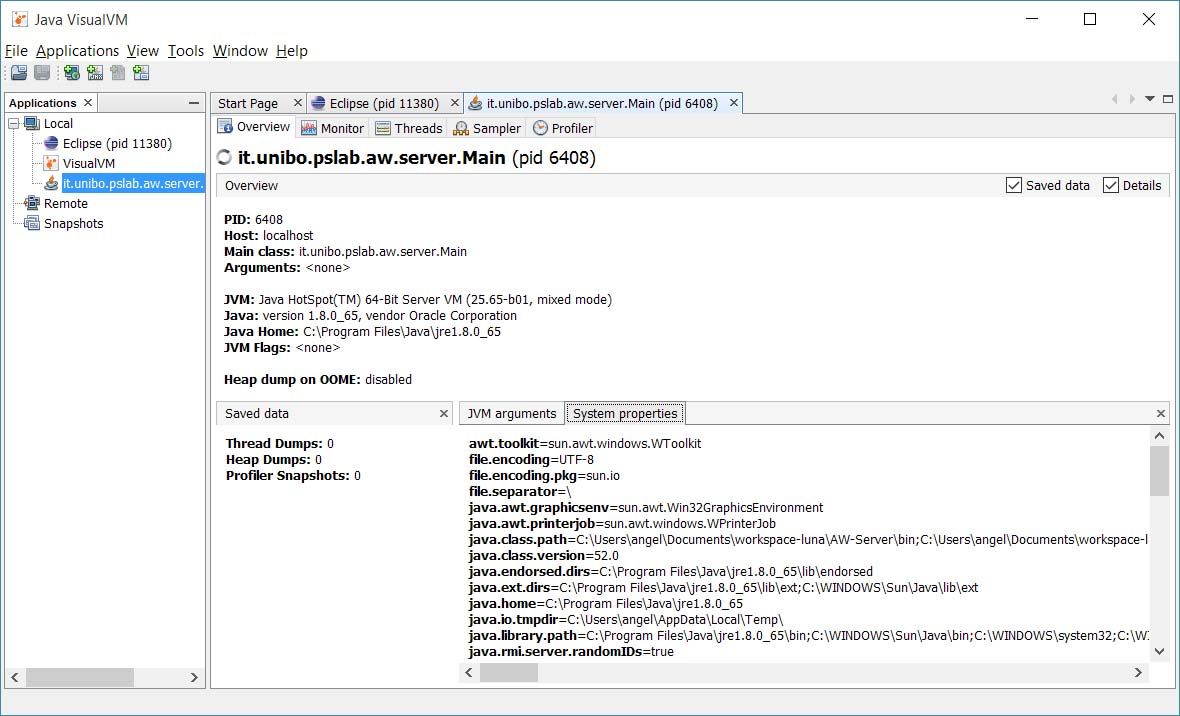
\includegraphics[width=0.99\textwidth]{img/jvisualvm-0}
\end{frame}

\begin{frame}{JVisualVM - Monitor}
\centering
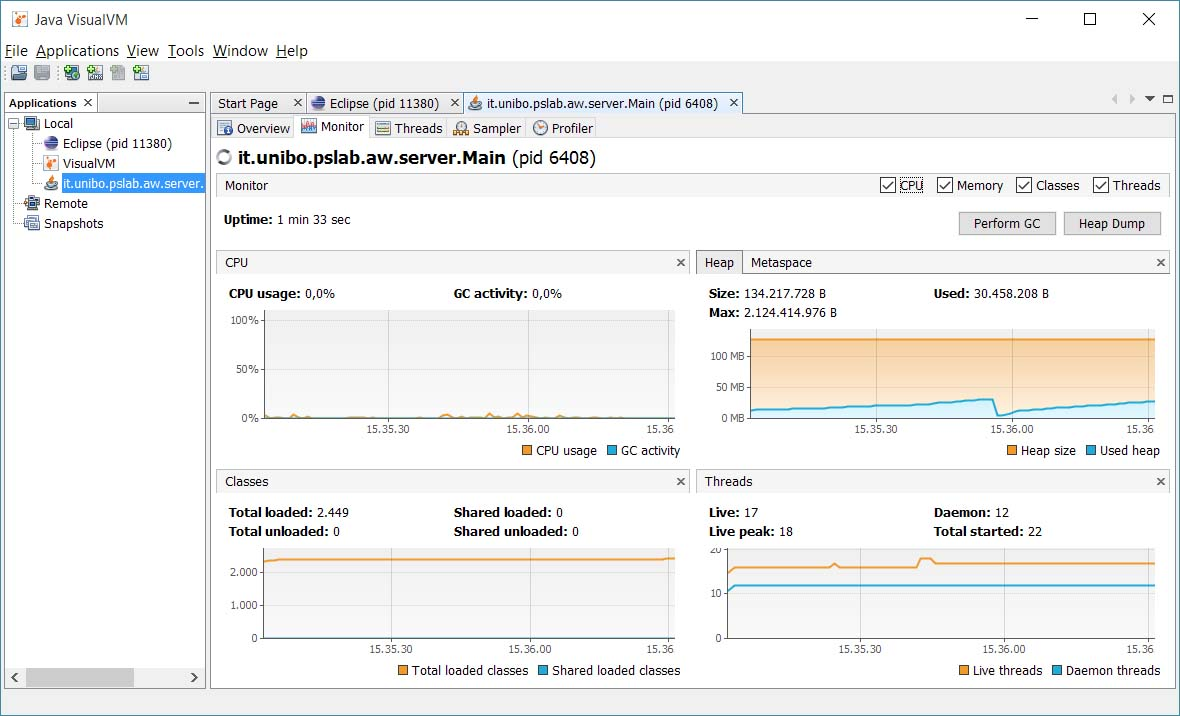
\includegraphics[width=0.99\textwidth]{img/jvisualvm-1}
\end{frame}

\begin{frame}{JVisualVM - Threads Status}
\centering
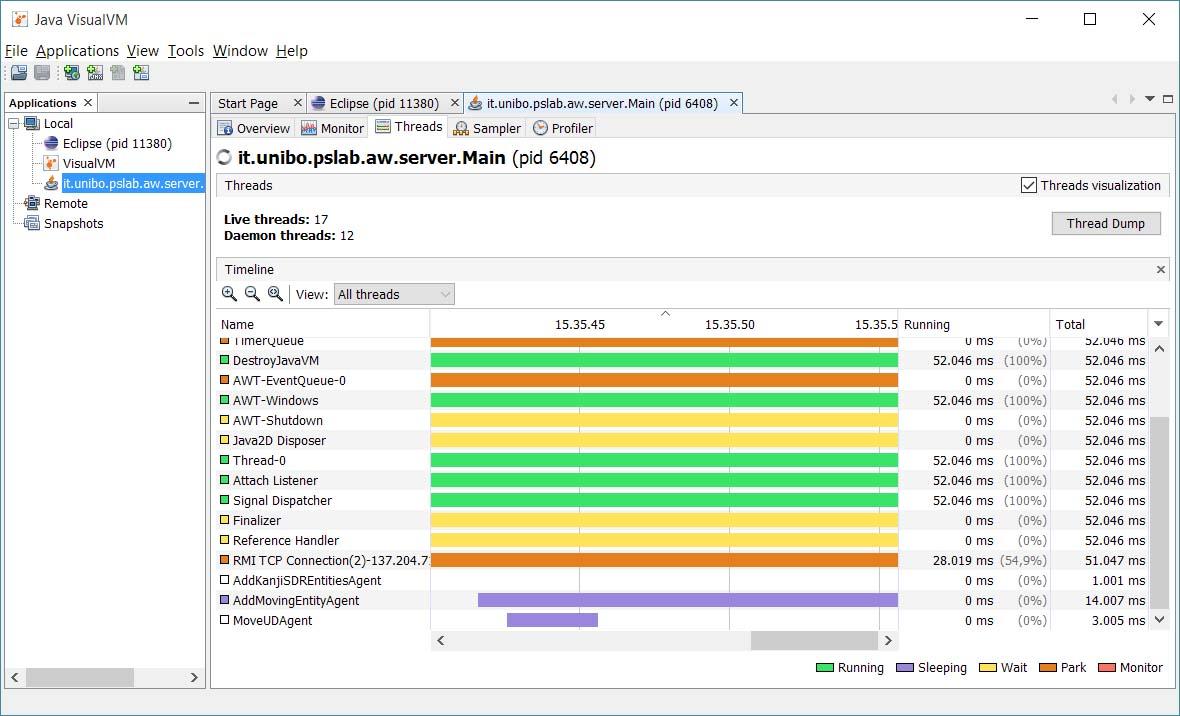
\includegraphics[width=0.99\textwidth]{img/jvisualvm-2}
\end{frame}

\begin{frame}{JVisualVM - Thread Dump Example}
\centering
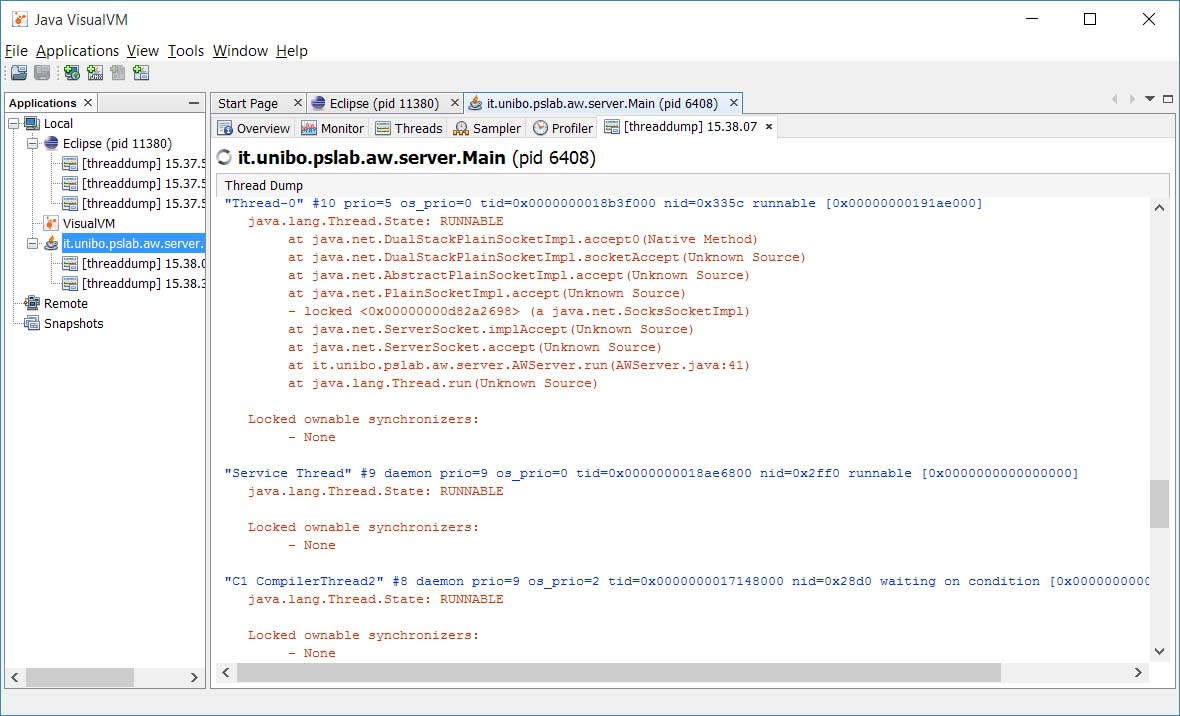
\includegraphics[width=0.99\textwidth]{img/jvisualvm-3}
\end{frame}

\subsection{GUI reattive}

\begin{frame}{Esercizi da svolgere in Autonomia}
\begin{block}{Esercizi sulle GUI reattive}
\begin{enumerate}
\item \emph{gui1}: studiare e analizzare il primo esercizio, aiutandosi con i commenti
\item \emph{gui2}: estensione di \emph{gui1} (seguire le istruzioni riportate nel test dell'esercizio)
\item \emph{gui3}: ulteriore estensione di \emph{gui3}
\end{enumerate}
\end{block}

\begin{block}{Esercizi sui Worker}
\begin{enumerate}
\item  \emph{worker1}: studiare e analizzare il primo esercizio, aiutandosi con i commenti
\item \emph{worker2}: estensione di \emph{worker1} (seguire le istruzioni riportate nel test dell'esercizio)
\end{enumerate}
\end{block}
\end{frame}

\begin{frame}{Approfondimenti}
\begin{block}{MVC per GUI reattive}
\begin{enumerate}
\item \emph{rguis.mvc}: presenta un esempio di implementazione di \emph{gui1} usando il pattern MVC. 
\item Consideratelo come un esempio di uso di MVC per la progettazione di GUI reattive!
\item Analizzarne e comprenderne struttura e comportamento.
\end{enumerate}
\end{block}

\end{frame}

\end{document}


\section{Monitoring e Debugging di Applicazioni Concorrenti}

\fr{Monitoring Thread: JConsole TOOL}{
	\bl{}{
	JConsole \cite{jconsole} is the Java Monitoring and Management Console, a graphical tool shipped in J2SE JDK 5.0 (and later versions)
		\iz{
			\item It uses the instrumentation of the Java virtual machine to provide information on performance and resource consumption of applications running on the Java platform
			\item Based on the Java Management Extension (JMX) technology
		}
	}
	\bl{}{
		Useful (also) to monitor the thread spawned by a running Java programs
		\iz{ \item Including VM threads, such as the one used for garbage collecting}
	}
}
\fr{Using JConsole 1/2}{
	\iz{ 
		\item JDK $<$ 1.6 start the Java application that you want to monitor with the option: 
			\iz{ 
				\item \cil{-Dcom.sun.management.jmxremote}
				\item e.g. \cil{java -Dcom.sun.management.jmxremote -cp bin Test}
			}
	}
	\iz{
		\item JDK $>=$ 1.6 it just type \cil{jconsole} from the command line
		\iz{ 
			\item When JConsole starts, you will be given a choice of all the Java applications that are running locally that JConsole can connect to
			\item Connections with remote applications is possible as well (e.g. \cil{jconsole hostName:portNum})
		}
	}
}
\fr{Using JConsole 2/2}{
	\fg{height=0.6\textheight}{img/jconsole.png} 
}
\fr{VisualVM: Am Open-Source Profiler}{
	\iz{
		\item Similar to JConsole, VisualVm \cite{visualvm} is a full-fledged profiler allowing to measure and visualize performances of Java programs
			\iz{
				\item It uses the instrumentation of the Java virtual machine to provide information on performance and resource consumption of applications running on the Java platform (like JConsole)
				\item Based on the Java Management Extension (JMX) technology
				\item Shipped with J2SE JDK 5.0 (and later versions)
			}
		}
	\iz{
		\item More fine-grained monitoring than JConsole
			\iz{
				\item Monitoring \% CPU used by methods, threads
				\item Monitoring how long a thread is blocked or running
				\item ...
			}
	}
}
\section{Somma Concorrente degli Elementi di un Array}

\fr{Concurrent Adder 1/3}{
	\bl{}{
		Vogliamo calcolare la somma di tutti gli elementi di un array (elevandoli prima al cubo) in maniera concorrente, sfruttando un certo insieme di worker thread
			\iz{
				\item Useremo come riferimento l'architettura del \textit{``concurrent sorter''} visto a lezione
				\item L'elevamento al cubo è stato introdotto semplicemente al fine di notare uno speedup tra la versione sequenziale e quella concorrente (vedere prossime slide)
			}
	}
	\bl{\cil{oop1314.lab09.adder.ConcurrentAdder}}{
		A tal fine renderemo concorrente l'implementazione di \cil{oop1314.lab09.adder.SequentialAdder} seguendo i passi riportati nelle prossime slide
	}
}

\fr{Concurrent Adder 2/3}{
	\bl{Passi da Seguire}{
		\en{
			\item Creare la classe \cil{ConcurrentAdder}
			\item Creare al suo interno l'inner static class \cil{AdderWorker} che estenderà la classe \cil{Thread}
			\item Creare il costruttore \cil{AdderWorker (long[] data, int minIndex, int maxIndex)} 
			\item Definire il campo \cil{long sum}
			\item Definire il metodo \cil{run} in \cil{AdderWorker} in cui memorizzare all'interno del campo \cil{sum} la somma elevata al cubo degli elementi di interesse
				\iz{\item Analogamente a quanto visto per il sorter concorrente}
			\item Definire il selettore \cil{public long getSum()} in modo che restituisca il valore del campo \cil{sum}
		}
	}
}

\fr{Concurrent Adder 3/3}{
	\bl{Passi da Seguire}{
		\en{
			\item Nel \cil{main} di \cil{ConcurrentAdder} istanziare un numero \cil{nWorker} di \cil{AdderWorker} pari a nCPU + 1
				\iz{\item nCPU va ricavando utilizzando il metodo statico \cil{Runtime.getRuntime().availableProcessors()}}
			\item Suddividere equamente il lavoro tra gli \cil{nWorker} (sempre nel \cil{main})
				\iz{\item Per semplicità, allocare all'ultimo worker eventuali elementi in eccesso derivanti da una suddivisione con resto degli elementi dell'input array}
			\item Stampare in stdout il tempo necessario ad effettuare la somma (sempre nel \cil{main})
				\iz{ \item Fare riferimento all'implementazione del main di \cil{SequentialAdder} per capire come calcolare il tempo}
		}
	}
	
}
\fr{Concurrent Adder: Testing}{
	\bl{Testing}{
		Lanciare il programma e confrontare i tempi di esecuzione tra la versione concorrente e quella sequenziale
			\iz{ \item Dovremmo sperimentare uno speedup del programma concorrente rispetto alla versione sequenziale}
	}
	
	\bl{Nota}{
		Se NON si dovesse notare lo speedup, è perché l'infrastruttura di virtualizzazione delle macchine del laboratorio non consente di ottenere dei risultati veritieri (il tempo puo' risultare inficiato da politiche di scheduling del server di virtualizzazione così come da ritardi dovuti alla rete): in questo caso, provare lo stesso test su una macchina fisica (anche a casa)
	}
}
\section{Costruzione di GUI Reattive}
%\section{Checksum di un File (Calcolato in Maniera Concorrente)}
\fr{SimpleReactiveGUI}{
	\bl{}{
		Saper sviluppare GUI reattive e responsive alle interazioni dell'utente è un aspetto di fondamentale importanza (come visto a lezione)
	}
	\bl{Obiettivo}{
		\iz{
			\item Rendere la GUI \cil{SimpleReactiveGUI} responsive all'interazione con un generico utente
			\item In particolare, \cil{SimpleReactiveGUI} dovrà consentire di salvare sul file system un array di 10 milioni di long contenente valori casuali, a seguito del click sul pulsante \cil{Save}
		}
	}
}

\fr{SimpleReactiveGUI 1/2}{
	\bl{Primo passo}{
		\iz{
			\item Implementare l'operazione di salvataggio su file system direttamente nel listener del pulsante \textit{Save}
			\item Fare il testing dell'applicazione: controllare che il comportamento atteso corrisponda a quello sperimentato 
		}
	}
	
	\bl{Secondo passo}{
		Risolvere i problemi relativi all'implementazione precedente introducendo un thread dedicato per il salvataggio su file
			\iz{
				\item Appoggiarsi alla creazione di un oggetto thread anonimo all'interno del listener relativo ai click sui bottoni
			}
		\sizedcode{\scriptsize}{code/Thread.java}
	}
}

\fr{SimpleReactiveGUI 2/2}{
	\bl{}{
		Che cosa succede se viene premuto una seconda volta il pulsante \cil{Save} prima che il salvataggio sul file system sia stato effettivamente completato?
			\iz{ \item Verificarlo in maniera autonoma tramite debugging}
	}

	\bl{}{
		Trovare in autonomia ad una soluzione per risolvere il problema
			\iz{ \item E' una soluzione molto semplice... non vogliamo più ricevere eventi dal bottone \cil{Save} fino a che... e ricominciare poi a riceverli nuovamente una volta che...}
	}
}

\section{Sfida tra Robot in un Ambiente Condiviso}
\fr{Object Search Contest 1/2}{
	\bl{Quali saranno i robot più veloci a trovare N oggetti nell'ambiente?}{
		Vogliamo costruire una competizione tra robot (software) per stabilire chi riesce ad individuare più velocemente un certo numero di oggetti
	}
	\bl{Punto di partenza: le classi in \cil{oop1314.lab09.robot}}{
		Cosa è cambiato
		\iz{
			\item \cil{RobotEnvironment}: è condiviso da tutti i robot e contiene al suo interno un dato numero (specificato nel costruttore) di oggetti recuperabili dai robot. Metodi aggiunti
				\iz{
					\item \cil{addRobot}: agginge un robot alla posizione specificata
					\item \cil{searchObjFromCurrPoistion}: per cercare un oggetto nelle vicinanze (robotX+-1,robotY+-1) di un robot
					\item \cil{pickObj}: per recuperare un oggetto alla posizione specificata
				}
			\item \cil{Robot}: modificata per allinearsi alle modifiche apportate a \cil{RobotEnvironment}, in particolare aggiunti i metodi \cil{searchObjFromCurrPoistion} e \cil{pick}
		}
	}
}

\fr{Object Search Contest 2/2}{
	\bl{}{
		Completare la classe \cil{RobotControllerAgent} che avrà il compito di governare in maniera autonoma il comportamento di un robot seguendo le indicazioni riportate nei commenti
		\iz{
			\item Ogni robot sarà quindi governato da un flusso di controllo indipendente, in competizione con gli altri
		}
	}
	
	\bl{}{
		Completare la classe \cil{TestingRobot} seguendo le indicazioni riportate nei commenti e lanciare il test
	}
}
\fr{Object Search Contest: Prime Modifiche}{
	\bl{}{
		Effettuando il testing del programma notiamo che vengono generate un insieme di eccezioni di tipo \textit{ConcurrentModificationException}
			\iz{ \item Perchè? Provare di capire il motivo in autonomia, analizzando il messaggio di erore ripotato}
	}
	\bl{}{
		Provare a risolvere in autonomia il problema, ricordando i costrutti di sincronizzazione visti a lezione
			\iz{\item La keyword \cil{synchronized} in particolare}
	}
	\bl{Testing}{
		Effettuare nuovamente il testing dell'applicazione per verificare la correttezza delle modifiche apportate
	}
}

\fr{Object Search Contest: Ulteriori Modifiche}{
	\bl{}{
		Miglioriamo la stampa dei rankings
			\iz{ \item In modo tale da non dover andare a cercare manualmente i messaggi in stdout }
	}
	\bl{Passi da seguire}{
		\iz{
			\item Completare la classe \cil{Ranker} seguendo le linee guida dei sorgenti, ricordandosi di utilizzare - quando necessario - opportuni meccanismi di sincronizzazione per evitare corse critiche
			\item Modificare il costruttore di \cil{RobotControllerAgent} come segue
				\iz{ \item \cil{RobotControllerAgent(Robot r, int nItemsToPick, Ranker ranker)} } 
			\item Nel metodo \cil{run} di \cil{RobotControllerAgent} appoggiarsi al ranker per notificare la terminazione delle operazioni di ricerca
			\item Nella classe \cil{TestingRobot} creare il ranker e passarlo ai vari controller, dopodiché quando tutti avranno terminato le ricerche, stampare la classifica appoggiandosi al metodo \cil{printRankings}
		}
	}
}

\section{Esercizi Aggiuntivi}
\fr{Ultimiamo l'implementazione di SimpleReactiveGUI}{
	\bl{}{
		Implementare l'handler del bottone \cil{Checksum} in modo tale che calcoli il checksum relativo al file \cil{data.dat} memorizzato dal bottone \cil{Save} e visualizzi tale risultato nella label visualizzata nella GUI
	}
	\bl{Nota}{
		Calcolare il checksum come semplice somma del valore di tutti i byte contenuti nel file \cil{data.dat}
	}
}

\begin{frame}[allowframebreaks]
 \frametitle{Bibliography}
	\bibliographystyle{plain}
	\small
 \bibliography{biblio}
\end{frame}

